%%%%%%%%%%%%%%%%%%%%%%%%%%%%%%%%%%%%%%%%%%%%%%%%%%%%%%%%%%%%%%%%%%%
%                                                                 %
%  GEANT manual in LaTeX form                              %
%                                                                 %
%  Michel Goossens (for translation into LaTeX)                   %
%  Version 1.00                                                   %
%  Last Mod. Jan 24 1991  1300   MG + IB                          %
%                                                                 %
%%%%%%%%%%%%%%%%%%%%%%%%%%%%%%%%%%%%%%%%%%%%%%%%%%%%%%%%%%%%%%%%%%%
\Origin {P.Zanarini}
\Documentation{P.Zanarini}
\Submitted{15.05.84}       \Revised{10.12.93}
\Version{Geant 3.16}\Routid{DRAW120}
\Makehead{Draw a volume cut view}
\Shubr{GDRAWX}{(CHNAME,CUTTHE,CUTPHI,CUTVAL,THETA,PHI,U0,V0,SU,SV)}
 
\begin{DLtt}{MMMMMMMM}
\item[CHNAME] ({\tt CHARECTER*4}) name of volume;
\item[CUTTHE] ({\tt REAL}) $\theta$ angle of the line normal to the cut plane;
\item[CUTPHI] ({\tt REAL}) $\phi$ angle of the line normal to the cut plane;
\item[TETHA]  ({\tt REAL}) viewing angle $\theta$;
\item[PHI]    ({\tt REAL}) viewing angle $\phi$;
\item[U0]     ({\tt REAL}) u coordinate on the screen of the volume origin;
\item[V0]     ({\tt REAL}) v  coordinate on the screen of the volume origin;
\item[SU]     ({\tt REAL}) scale factor for u  coordinates;
\item[SV]     ({\tt REAL}) scale factor for v   coordinates.
\end{DLtt}

Draws a {\it cut view} of the volume {\tt CHNAME}
with all its {\it visible} descendants, i.e. draws their intersection with
the cut plane normal to the axis
given by the angles {\tt CUTTHE, CUTPHI} at the distance {\tt CUTVAL}
from the origin.
The view point is defined by the angles {\tt THETA, PHI}.
{\tt U0, V0, SU, SV} have the same meaning as in \Rind{GDRAW}.
These {\it view parameters}, as well as zoom parameters set by \Rind{GDZOOM}
are copied in \FCind{/GCDRAW/}.

Attributes like colour, surface fill, line width, line style, visibility, etc.
can be set by the \Rind{GSATT} routine for {\tt CHNAME}
and its descendants {\tt [GEOM500]}.
 
\Shubr{GDRAWC}{(CHNAME,IAX,CUTVAL,U0,V0,SU,SV)}
 
\begin{DLtt}{MMMMMMMM}
\item[CHNAME] ({\tt CHARECTER*4}) name of volume;
\item[IAX]  ({\tt INTEGER}) axis of the cut (1=X, 2=Y, 3=Z);
\item[U0]   ({\tt REAL}) u coordinate on the screen of the volume origin;
\item[V0]   ({\tt REAL}) v coordinate on the screen of the volume origin;
\item[SU]   ({\tt REAL}) scale factor for u coordinates;
\item[SV]   ({\tt REAL}) scale factor for v coordinates.
\end{DLtt}

This routine is a special case of the previous \Rind{GDRAWX}.
Here the cut plane is normal to one of the main axes ({\tt IAX})
and placed at a distance {\tt CUTVAL} from the origin.
The view-point is along the same axis.
 
Fig.~\ref{fg:draw120-1} gives an example of utilisation of 
\Rind{GDAXIS}, \Rind{GDRAW} and \Rind{GDRAWX}. Fig.~\ref{fg:draw120-2}
gives an example of use of \Rind{GDRAWC}.

\begin{figure}[hbt]
     \centering
     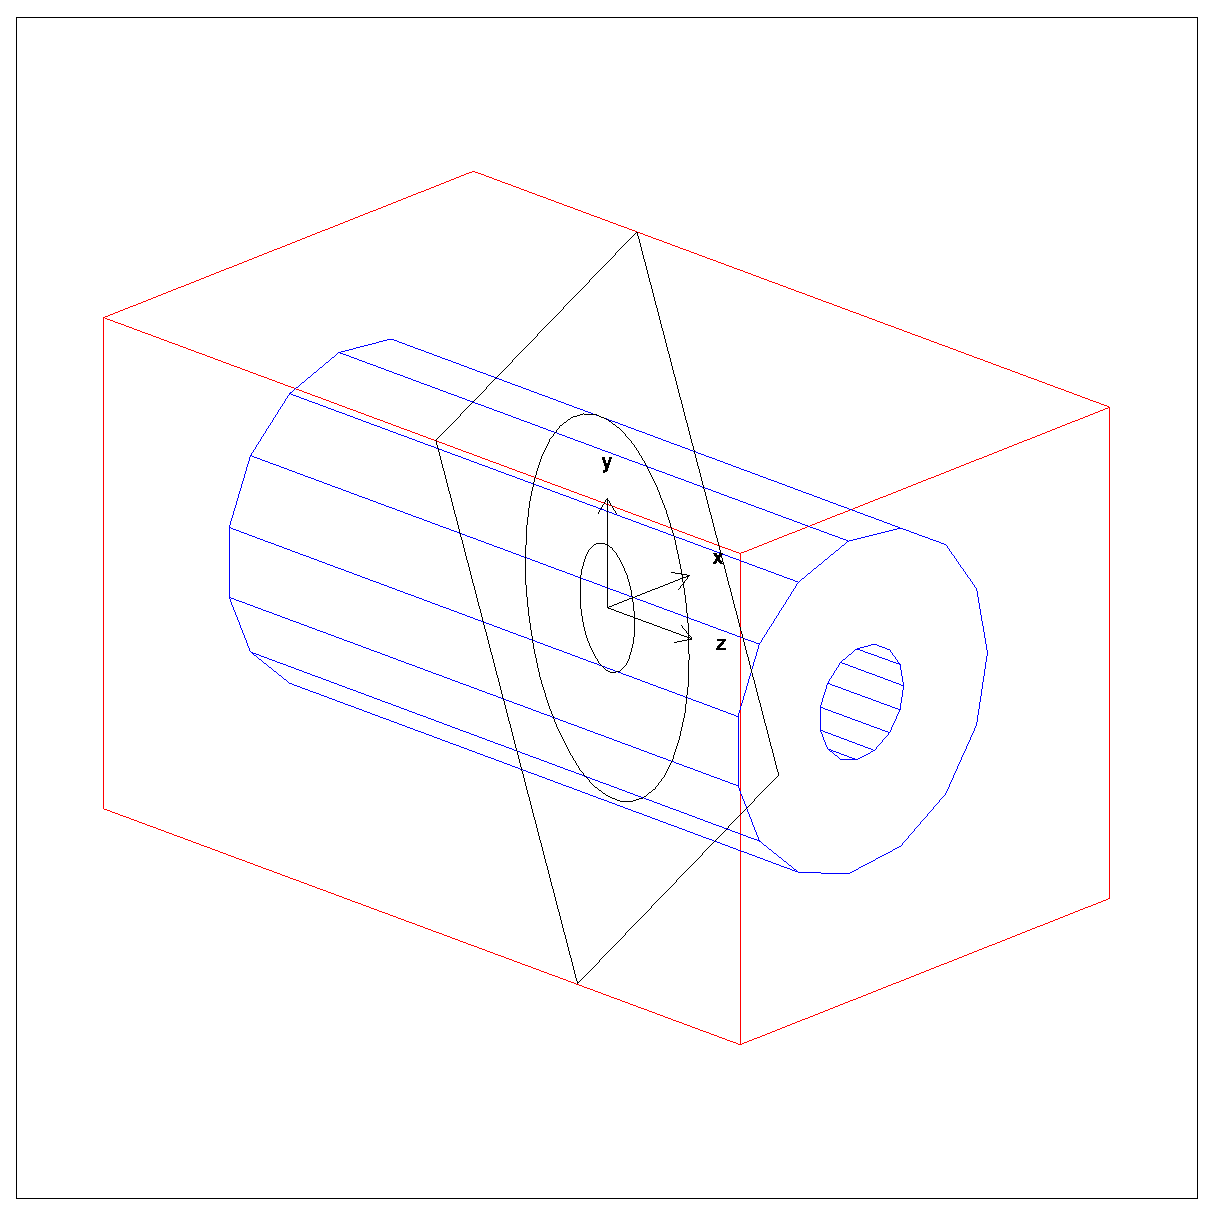
\epsfig{file=eps/draw120-1.eps,width=14cm}
\begin{verbatim}
      CALL GDOPT('HIDE','ON')
      CALL GSATT('NBOX','COLO',2.)
      CALL GSATT('NTUB','COLO',4.)
      CALL GDRAW('NBOX',50.,150.,0.,10.,10.,0.01,0.01)
      CALL GDRAW('NTUB',50.,150.,0.,10.,10.,0.01,0.01)
      CALL GDOPT('HIDE','OFF')
      CALL GSATT('*','COLO',1.)
      CALL GDRAWX('NBOX',30.,40.,0.,50.,150.,10.,10.,0.01,0.01)
      CALL GDAXIS(0.,0.,0.,200.)
\end{verbatim}
     \caption{Example of utilisation of 
{\tt GDAXIS}, {\tt GDRAW} and {\tt GDRAWX}}
     \label{fg:draw120-1}
\end{figure}
 
\begin{figure}[hbt]
     \centering
     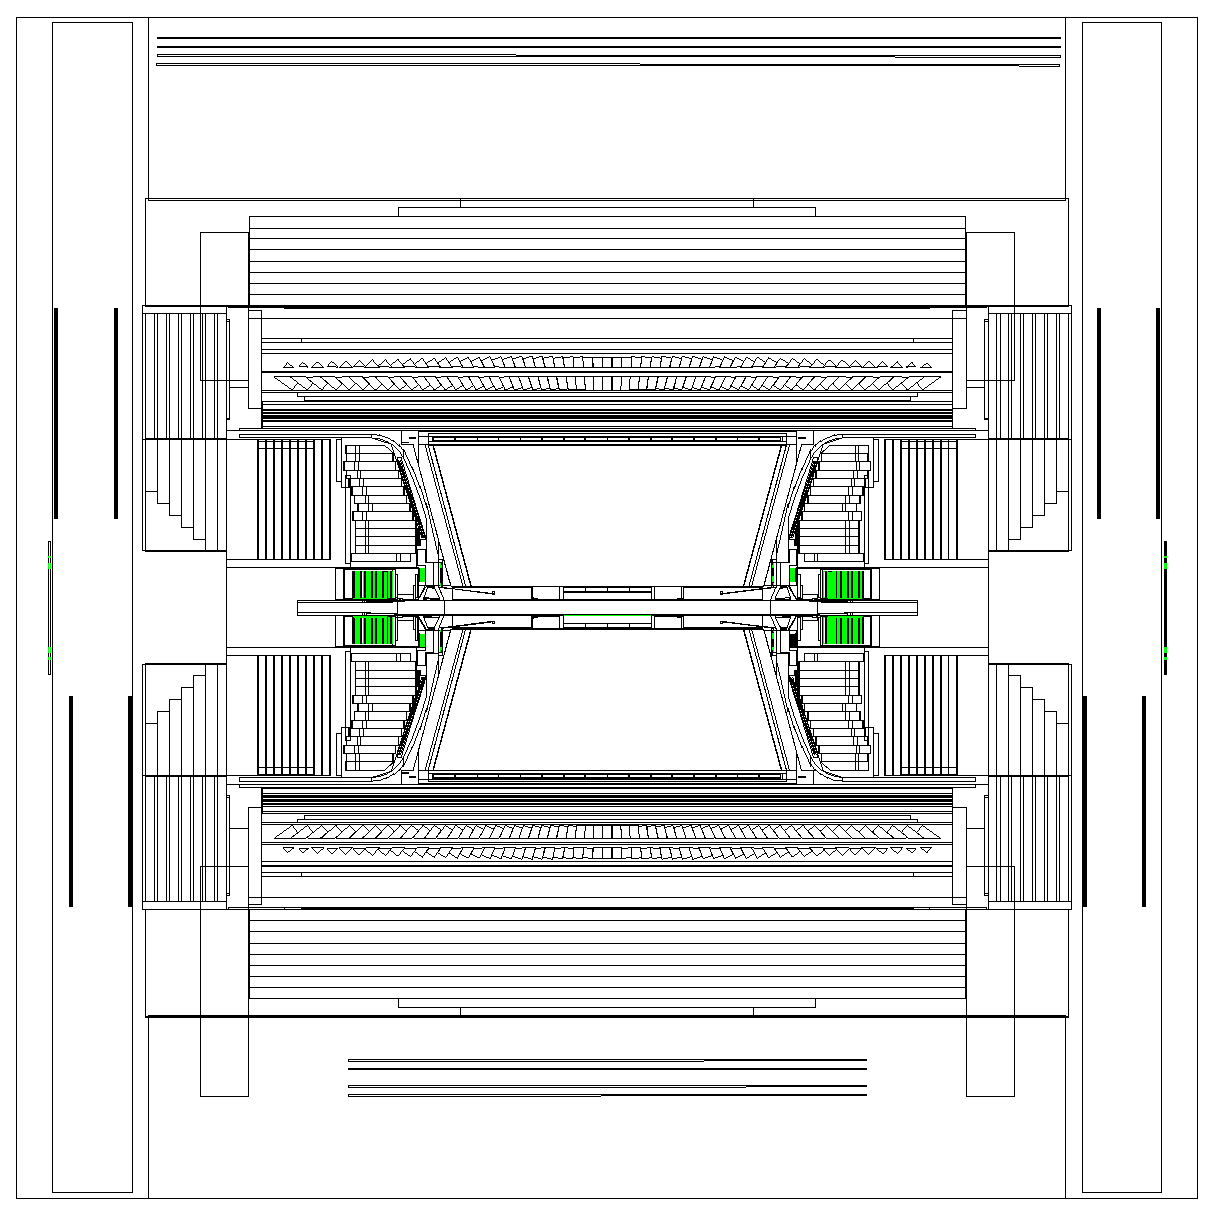
\epsfig{file=eps/draw120-2.eps,width=14cm}
\begin{verbatim}
      CALL GDRAWC('OPAL',2,0.,10.,10.,0.01,0.01)
\end{verbatim}
     \caption{Example of utilisation of {\tt GDRAWC}}
     \label{fg:draw120-2}
\end{figure}
